\chapter{Sommatori, complemento a 2 e codici}
\label{ch:sommatori}

\section{Esempio: sommatore a 4 bit}
\textit{(27 marzo 2026)}

Collegando in cascata 4 sommatori completi (Full Adder, FA) si ottiene un circuito per l'addizione a 4 bit, noto come \textbf{Ripple-Carry Adder} (sommatore a propagazione di riporto). Ogni stadio $i$ somma i bit $a_i$ e $b_i$ più il riporto dello stadio precedente ($C_i$), generando il bit di somma ($\Sigma_i$) e il nuovo riporto ($C_{i+1}$) per lo stadio successivo.

\begin{center}
\begin{circuitikz}[scale=0.72, every node/.style={scale=0.72}]
% 4 FA in cascata
\foreach \i/\xi in {0/0, 1/2.6, 2/5.2, 3/7.8}{
  \draw (\xi,0) rectangle (\xi+2.0, 1.8);
  \node at (\xi+1.0, 0.9) {FA};
}
% Ingressi a_i
\foreach \i/\xi/\lab in {0/0/$a_0$, 1/2.6/$a_1$, 2/5.2/$a_2$, 3/7.8/$a_3$}{
  \draw[-latex] (\xi+0.6, 2.4) -- (\xi+0.6, 1.8) node[midway,right,font=\small]{\lab};
}
% Ingressi b_i
\foreach \i/\xi/\lab in {0/0/$b_0$, 1/2.6/$b_1$, 2/5.2/$b_2$, 3/7.8/$b_3$}{
  \draw[-latex] (\xi+1.4, 2.4) -- (\xi+1.4, 1.8) node[midway,right,font=\small]{\lab};
}
% Carry chain: C0 entra da sinistra, C1..C4 si propagano
\draw[-latex] (-1.0, 0.9) -- (0, 0.9) node[midway,above,font=\small]{$C_0$};
\draw[-latex] (2.0,0.9) -- (2.6,0.9) node[midway,above,font=\small]{$C_1$};
\draw[-latex] (4.6,0.9) -- (5.2,0.9) node[midway,above,font=\small]{$C_2$};
\draw[-latex] (7.2,0.9) -- (7.8,0.9) node[midway,above,font=\small]{$C_3$};
\draw[-latex] (9.8,0.9) -- (10.5,0.9) node[right,font=\small]{$C_4$};
% Uscite Sigma
\foreach \i/\xi/\lab in {0/0/$\Sigma_0$, 1/2.6/$\Sigma_1$, 2/5.2/$\Sigma_2$, 3/7.8/$\Sigma_3$}{
  \draw[-latex] (\xi+1.0, 0) -- (\xi+1.0,-0.6) node[below,font=\small]{\lab};
}
% Freccia overflow su C4
\draw[-latex,color=teal] (10.5,0.9) -- ++(0.5,0.4) node[right,font=\small,color=teal]{\textbf{bit di overflow}};
\end{circuitikz}
\end{center}

\medskip
\textbf{Esempio rapido di calcolo:}\\
Proviamo a sommare $A = 0101_2$ ($5_{10}$) e $B = 0011_2$ ($3_{10}$), ponendo il riporto iniziale $C_0 = 0$:
\begin{itemize}
    \item \textbf{Stadio 0:} $a_0(1) + b_0(1) + C_0(0) = 2 \implies \Sigma_0 = 0$, riporto $C_1 = 1$.
    \item \textbf{Stadio 1:} $a_1(0) + b_1(1) + C_1(1) = 2 \implies \Sigma_1 = 0$, riporto $C_2 = 1$.
    \item \textbf{Stadio 2:} $a_2(1) + b_2(0) + C_2(1) = 2 \implies \Sigma_2 = 0$, riporto $C_3 = 1$.
    \item \textbf{Stadio 3:} $a_3(0) + b_3(0) + C_3(1) = 1 \implies \Sigma_3 = 1$, riporto $C_4 = 0$.
\end{itemize}
Risultato corretto: $\Sigma = 1000_2$ ($8_{10}$).

\begin{definizione}{Bit di overflow $C_4$}
\textbf{Bit di overflow} ($C_4$): è il bit di riporto finale in uscita dal blocco più significativo. Se stiamo eseguendo addizioni su numeri binari puri (senza segno) a 4 bit e otteniamo $C_4 = 1$, il risultato supera il valore massimo rappresentabile ($15_{10}$). In questo caso si è verificato un errore di overflow.
\end{definizione}

\textbf{Il problema del ritardo (Delay):}\\
Il principale limite prestazionale di questo circuito è che ogni blocco FA deve "aspettare" che il blocco precedente calcoli il suo riporto. Il segnale $C$ deve letteralmente "propagarsi" a cascata (ripple) da $C_0$ fino a $C_4$. 
\begin{itemize}
    \item Se una singola porta logica ha un tempo di ritardo $\Delta T$, ogni blocco Full Adder impiega circa $3\Delta T$ per generare il riporto.
    \item In un sommatore a $n$ bit, il tempo totale $\Delta t$ cresce in modo lineare:
    \[ \Delta t = n \cdot 3\Delta T \]
\end{itemize}

\textbf{Soluzione: i sommatori Carry Look-Ahead (CLA)}\\
Per eliminare questa latenza si utilizzano circuiti più avanzati (ad anticipo di riporto). Attraverso un'apposita rete logica parallela, questi circuiti capiscono "in anticipo" se i vari stadi andranno a \emph{generare} o \emph{propagare} un riporto. In questo modo si possono calcolare tutte le uscite simultaneamente, con un ritardo bassissimo e logaritmico (o indipendente) rispetto alla lunghezza $n$ della parola.

\section{Modularità e Design Gerarchico}

Nella progettazione digitale moderna, si sfrutta ampiamente il concetto di \textbf{modularità}.

\begin{definizione}{Design Modulare}
un approccio in cui il sistema complesso viene suddiviso in sottomoduli standard e interscambiabili (es. usare i Full Adder base per costruire un sommatore a $n$ bit). Questi moduli possono essere aggiunti, rimossi o sostituiti senza dover alterare o riprogettare il resto del sistema.
\end{definizione}

\noindent I vantaggi principali includono:
\begin{itemize}
    \item \textbf{Astrazione}: chi progetta un processore non deve preoccuparsi della logica a porte interne al singolo FA, ma ne considera solo gli ingressi e le uscite.
    \item \textbf{Riutilizzo e Semplificazione}: un modulo testato e verificato può essere riutilizzato in più punti, rendendo il collaudo molto più affidabile.
\end{itemize}

\section{Sottrattori e numeri negativi}
\textit{(27 marzo 2026 -- cont.)}

Nei circuiti digitali, per rappresentare anche i numeri negativi, si deve "sacrificare" un bit (di solito il più significativo) per indicare il segno. Esistono diverse tecniche per farlo:

\textbf{1. Modulo e Segno}\\
Il bit più a sinistra indica il segno ($0$ = positivo, $1$ = negativo), mentre i restanti bit indicano il valore assoluto. Questa tecnica presenta un problema pratico: lo zero ha due rappresentazioni diverse. Ad esempio su 4 bit, $0000$ ($+0$) e $1000$ ($-0$) indicano entrambi il numero zero. Questo complica inutilmente i circuiti di calcolo.

\textbf{2. La teoria dei Complementi}\\
Per risolvere questo problema si utilizza un metodo matematico chiamato \emph{complemento}. Dato un numero $N$ espresso in una certa base $r$ e lungo $n$ cifre, si definiscono due tipi di complemento:
\begin{itemize}
    \item \textbf{Complemento alla base diminuita (base $r-1$):} \\
    Si definisce come $C_{r-1}(N) = (r^n - 1) - N$. Poiché $r^n - 1$ è il numero massimo rappresentabile ($N_{\max}$), si ottiene sottraendo il numero $N$ dal valore massimo.
    \item \textbf{Complemento alla base (base $r$):} \\
    Si definisce come $C_r(N) = r^n - N$. Essendo $r^n = (r^n - 1) + 1$, equivale matematicamente ad aggiungere $1$ al complemento alla base diminuita.
\end{itemize}

\textbf{Applicazione al Sistema Binario (Base 2):}\\
Nei sistemi binari (base $r=2$), queste due definizioni prendono il nome di \textbf{Complemento a 1} e \textbf{Complemento a 2}.

\textbf{Complemento a 1 ($C_1$):}
\[ C_1(N) = (2^n - 1) - N \]
Poiché $2^n-1$ è un numero composto da tutti "1" (es. $1111_2$), sottrarre $N$ significa banalmente \emph{invertire tutti i singoli bit} di $N$ (ogni bit $N_i$ diventa $\overline{N}_i$):
\[ C_1(N) = \overline{N}_{n-1}\cdots\overline{N}_1\overline{N}_0 \]

\textbf{Complemento a 2 ($C_2$):}
\[ C_2(N) = 2^n - N \]
Come visto prima, possiamo riscriverlo come $(2^n - 1 - N) + 1$. Questo significa che per calcolare il complemento a 2 basta prendere il complemento a 1 e sommare 1:
\[ C_2(N) = C_1(N) + 1 = \overline{N}_{n-1}\cdots\overline{N}_1\overline{N}_0 + 1 \]

\noindent\textit{Proprietà fondamentale:} Applicare due volte il complemento a 2 restituisce il numero originale, ovvero $C_2(C_2(N)) = N$.

\begin{definizione}{Complemento a 2}
Il \textbf{complemento a 2} è la notazione standard per rappresentare numeri interi con segno nei calcolatori. A differenza della codifica a modulo e segno, garantisce un'unica rappresentazione per lo zero (es. $0000$) e permette di eseguire somme e sottrazioni con la stessa rete logica hardware.
\end{definizione}

\noindent\textbf{Regola pratica per calcolare il complemento a 2 di un numero}:
\begin{enumerate}
    \item Si parte dal numero binario positivo (es. $+3_{10} = 0011_2$).
    \item Si invertono tutti i bit (complemento a 1): $0011 \to 1100$.
    \item Si somma $1$ al risultato: $1100 + 1 = 1101$. 
\end{enumerate}
Quindi $-3_{10} = 1101_2$ in complemento a 2 su 4 bit.

\medskip
Se verifichiamo calcolando l'addizione $-3 + 3$, avremo: $1101 + 0011 = 1\,0000$. Poiché lavoriamo a 4 bit, l'uno più a sinistra (il \emph{carry out} uscente) cade fuori dalla dimensione dei registri e viene ignorato. Il risultato memorizzato è esattamente $0000$, ovvero 0.

\subsection{Circuito sommatore/sottrattore a 4 bit}

Un grande vantaggio della codifica in complemento a 2 è la possibilità di eseguire sia addizioni che sottrazioni utilizzando il \textbf{medesimo circuito hardware}. Per farlo, si estende il classico sommatore (ripple-carry adder) introducendo delle porte logiche XOR sugli ingressi del secondo operando e sfruttando il riporto iniziale $C_0$ come segnale di controllo (selettore d'operazione).

\begin{center}
\begin{circuitikz}[scale=0.9, every node/.style={scale=0.9}]
\tikzset{FA/.style={draw, minimum width=1.6cm, minimum height=1.6cm, align=center}}

% Disegno dei 4 blocchi Full Adder
\foreach \i/\x in {0/0, 1/3.5, 2/7.0, 3/10.5} {
    \node[FA] (FA\i) at (\x,0) {FA$_\i$};
}

% Linea comune per C0 (selezione operazione)
\coordinate (C0line) at (-1.5, 4.0);
\draw (-1.5, 4.0) node[left] {$C_0$ (\textsf{0}=Add, \textsf{1}=Sub)} -- (11.0, 4.0);

% Connessione C0 come riporto in ingresso del primo FA
\draw[-latex] (-1.5, 4.0) -- (-1.5, 0) -- (FA0.west) node[midway, above] {$C_0$};

\foreach \i in {0,1,2,3} {
    % a_i input
    \draw[-latex] (FA\i.120 |- 0, 4.8) node[above] {$a_\i$} -- (FA\i.120);
    
    % b_i input e XOR
    \node[xor port, rotate=-90, scale=0.7] (XOR\i) at (FA\i.60 |- 0, 2.5) {};
    \draw[-latex] (XOR\i.out) -- (FA\i.60);
    
    % Connessione di b_i all'ingresso 1 dello XOR
    \draw (XOR\i.in 1) -- (XOR\i.in 1 |- 0, 4.8) node[above] {$b_\i$};
    
    % Connessione di C0 all'ingresso 2 dello XOR
    \draw (XOR\i.in 2) -- (XOR\i.in 2 |- C0line) node[circle, fill, inner sep=1.2pt] {};
}

% Carry chain tra i FA
\draw[-latex] (FA0.east) -- (FA1.west) node[midway, above] {$C_1$};
\draw[-latex] (FA1.east) -- (FA2.west) node[midway, above] {$C_2$};
\draw[-latex] (FA2.east) -- (FA3.west) node[midway, above] {$C_3$};

% Uscita C4
\draw[-latex] (FA3.east) -- ++(1.5,0) coordinate (C4out) node[above] {$C_4$};

% Uscite Somma (Sigma)
\foreach \i in {0,1,2,3} {
    \draw[-latex] (FA\i.south) -- ++(0,-1.0) node[below] {$\Sigma_\i$};
}

% XOR finale per l'overflow (E)
\node[xor port, scale=0.8] (E_XOR) at (13.5, -2.0) {};

% Preleviamo C3
\coordinate (tapC3) at (8.75, 0);
\draw (tapC3) node[circle, fill, inner sep=1.2pt] {} |- (E_XOR.in 2);

% Preleviamo C4
\coordinate (tapC4) at (12.0, 0);
\draw (tapC4) node[circle, fill, inner sep=1.2pt] {} |- (E_XOR.in 1);

\draw[-latex] (E_XOR.out) -- ++(0.8,0) node[right] {$E_{Overf}$};

\end{circuitikz}
\end{center}

Il funzionamento del circuito dipende dal valore del segnale di controllo $C_0$:

\begin{itemize}[leftmargin=1.5em]
    \item \textbf{Se $C_0=0$ (Addizione)}: la porta XOR riceve uno 0 e si comporta come un buffer trasparente ($b_i \oplus 0 = b_i$). Inoltre, il riporto in ingresso al primo FA è anch'esso 0. Il circuito esegue quindi una normale addizione: $S = a + b$.
    
    \item \textbf{Se $C_0=1$ (Sottrazione)}: la porta XOR riceve un 1 e si comporta come un invertitore logico ($b_i \oplus 1 = \overline{b}_i$), calcolando il complemento a 1 di $b$. Il riporto in ingresso al primo FA fornisce un ulteriore $+1$. In questo modo, il circuito calcola internamente l'espressione $a + \overline{b} + 1$. Poiché $\overline{b} + 1$ equivale a $-b$ (in complemento a 2), l'operazione totale svolta è esattamente la sottrazione: $S = a - b$.
    
    \item \textbf{Errore di Overflow ($E$)}: lavorando con un numero fisso di bit (in questo caso 4 bit, intervallo rappresentabile da $-8$ a $+7$), può accadere che il risultato reale dell'operazione sia al di fuori di questo intervallo. Questo errore prende il nome di \emph{overflow} e viene segnalato tramite una porta XOR applicata agli ultimi due riporti generati ($E = C_3 \oplus C_4$). Se $E=1$, si ha un \emph{overflow} e il risultato non è valido.
\end{itemize}

In generale, lavorando in complemento a 2 con 4 bit, si rappresenta l'intervallo da $-8$ a $+7$:
\begin{itemize}[leftmargin=1.5em]
    \item[\small$\blacksquare$] Se $\Sigma_3 = 0 \;\Leftrightarrow\;$ il risultato $\Sigma$ è positivo o nullo.
    \item[\small$\blacksquare$] Se $\Sigma_3 = 1 \;\Leftrightarrow\;$ il risultato $\Sigma$ è negativo.
\end{itemize}
Queste due regole valgono solo in assenza di overflow ($E=0$). Il segnale $E=C_3\oplus C_4$ ha senso per i numeri \emph{con segno}. Per una somma di numeri senza segno ($C_0=0$, intervallo $[0,15]$) l'overflow è segnalato direttamente da $C_4=1$.

\begin{center}
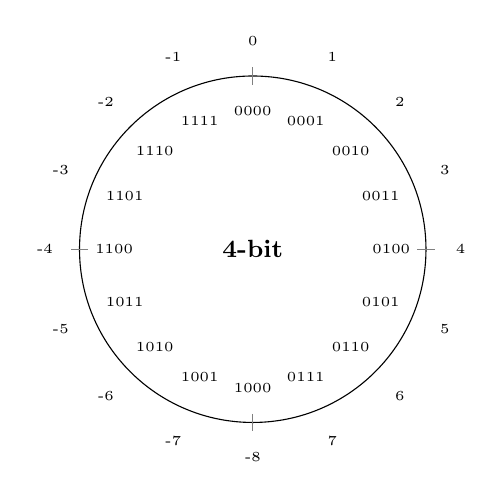
\begin{tikzpicture}[scale=1.1]
% Cerchio complemento a 2 a 4 bit
\draw (0,0) circle (2.0cm);
\foreach \angle/\val/\bin in {
  90/0/0000, 67.5/1/0001, 45/2/0010, 22.5/3/0011,
  0/4/0100, -22.5/5/0101, -45/6/0110, -67.5/7/0111,
  -90/-8/1000, -112.5/-7/1001, -135/-6/1010, -157.5/-5/1011,
  180/-4/1100, 157.5/-3/1101, 135/-2/1110, 112.5/-1/1111
}{
  \node[font=\tiny] at ({2.4*cos(\angle)},{2.4*sin(\angle)}) {\val};
  \node[font=\tiny] at ({1.6*cos(\angle)},{1.6*sin(\angle)}) {\bin};
}
\node[font=\small\bfseries, align=center] at (0,0) {4-bit};
% assi cardinali
\foreach \a in {0,90,180,270}{
  \draw[gray,thin] ({1.9*cos(\a)},{1.9*sin(\a)}) -- ({2.1*cos(\a)},{2.1*sin(\a)});
}
\end{tikzpicture}
\end{center}

% ======================================================================
\section*{Riepilogo del Capitolo}

\begin{important}
Il \textbf{complemento a 2} è lo standard per rappresentare i numeri con segno perché garantisce un'unica rappresentazione dello zero e permette di eseguire somma e sottrazione con lo stesso hardware (sommatore ripple-carry più una rete di XOR di controllo).
\end{important}

\begin{note}
\textbf{Formule fondamentali:}
\begin{itemize}
    \item \textbf{Complemento alla base e alla base diminuita:} $C_{r-1}(N) = (r^n-1)-N$; $\; C_r(N) = r^n - N$.
    \item \textbf{Complemento a 1:} inversione bit a bit, $C_1(N) = \overline{N}_{n-1}\cdots\overline{N}_0$.
    \item \textbf{Complemento a 2:} $C_2(N) = C_1(N)+1$, con la proprietà $C_2(C_2(N))=N$.
    \item \textbf{Sommatore/sottrattore a 4 bit:} XOR sugli ingressi $b_i$ controllati da $C_0$ ($C_0=0$ somma, $C_0=1$ sottrazione: $a+\overline{b}+1=a-b$).
    \item \textbf{Overflow:} con segno $E = C_3\oplus C_4$; senza segno $= C_4$.
    \item \textbf{Ritardo del ripple-carry a $n$ bit:} $\Delta t = n\cdot 3\Delta T$ (limite superato dai Carry Look-Ahead).
\end{itemize}
\end{note}

